\section{Discovery: an architectural proposal}
\label{sec:architecture}

\subsection{Related work}

% \begin{itemize}

% 	\item Moreno made a proposition of IaaS architecture \cite{moreno2012iaas}.	
	
% 	\item He identified a list of services that are vital for building IaaS that will be usable in production condition for commercial company.

% 	\item We aim at making a research prototype: we want to keep concepts that are vital for a first prototype:

% 		\begin{description}

% 			\item [Virtual Machine] : Prototype will enable reasearchers to access a big compute power.

% 			\item [Virtual Network] : In addition to infrastructure network, we want to connect virtual machines on an isolated network.

% 			\item [Image disk and persistent storage] : 
% 				\begin{itemize}

% 					\item Virtual machines will be based on images

% 					\item Virtual machines' states are savable.
				
% 				\end{itemize}

% 			\item [Simple authentication] : User will have to authenticate to access prototype. Once they are authenticated they will be able to create virtual machines.

% 		\end{description}

% \end{itemize}


In a recent study, authors have proposed a reference architecture for 
a Cloud OS \cite{moreno2012iaas}: they aimed at providing abstractions of 
underlying technologies that compose current IaaS managers. The strength of 
their work resides in the fact that they considered all the needs of an 
"industrial class" IaaS manager: each of its functions has been widely studied.
Beacause we find this work well detailed, we have decided that a new 
architectural proposition for a distributed IaaS manager should leverage this 
work.

However, since we aim at making a research prototype of a massively distributed
cloud, some parts of this reference architecture are outiside the scope of a 
research prototype. That is why we will volontarily neglect advanced services in
order to focus on those that can be considered as vitals, enabling us to propose
an architecure for a simple but working massively distributed IaaS manager. We 
also keep in mind that the architecture should be flexible enough to later 
include these advanced services in a painless way.

This first iteration on the LUC-OS will allow users to manage interconnected 
virtual machines (virtual environment). For this purpose we only keep services 
that are for use. To determine which services are needed, we
have listed concepts that are fundamentals for managing virtual machines:

\label{cloud_os_concepts}

\begin{description}

	\item [Virtual Machine] : Virtual machines is the key concept with regard to
	the system we aim to build. We can draw an analogy with computing ressources
	production between the LUC-OS and modern operating systems: in the same way 
	a modern  operating systems provides computing resources by provisioning 
	thread, the LUC-OS will produce virtual machines.

	\item [Virtual Network] : Virtual machines of a same virtual 
	environment need to be interconnected. This interconnection will be
	performed by means of virtual networks.

	\item [Image disk and persistent] : Virtual machines are based on 
	specified at creation disk images, leading to the point that the LUC-OS must
	propose a storage services for storing reference disk images. Furthermore a 
	virtual machine can be snapshotted, meaning that the LUC-OS must provides 
	efficient mechanisms for persisting these states.

	\item [Simple authentication] : As virtual machines provisioning is
	invocked by users, an authentication process is needed to guarantee that
	unregistered users cannot access resource allocation. This authentication 
	process will also have to handle user's role such as customer and LUC-OS's
	administrator.

\end{description}





\subsection{First iteration on the LUC-OS architecture}

% \begin{itemize}

% 	\item For our first iteration, we keep 4 main services:
% 		\begin{description}

% 			\item [Compute manager] : responsible for virtual machines lifecycle.

% 			\item [Network manager] : responsible for virtual networks.

% 			\item [Storage manager] : responsible for images and persistent block storage.

% 			\item [Administrative manager] : responsible for infrastructure management and user permissions.  

% 		\end{description}


% 	\item In figure \ref{fig:mcd} we propose a conceptual data model to explain our proposal.




% 	\item Virtual environment concept is the keystone of the Discovery proposal:
		
% 		\begin{itemize}

% 			\item When a user request the creation of virtual machines for a specified date, an allocation is registered.

% 			\item When the start date is reached, a virtual environment (isolated container for a VLAN and VMs) is created.

% 			\item a virtual environment can be run on several hosts, possibly spread over several geographical sites.

% 		\end{itemize}

% 	\item + description of other entities.

% \end{itemize}

\begin{figure*}
	\centering
	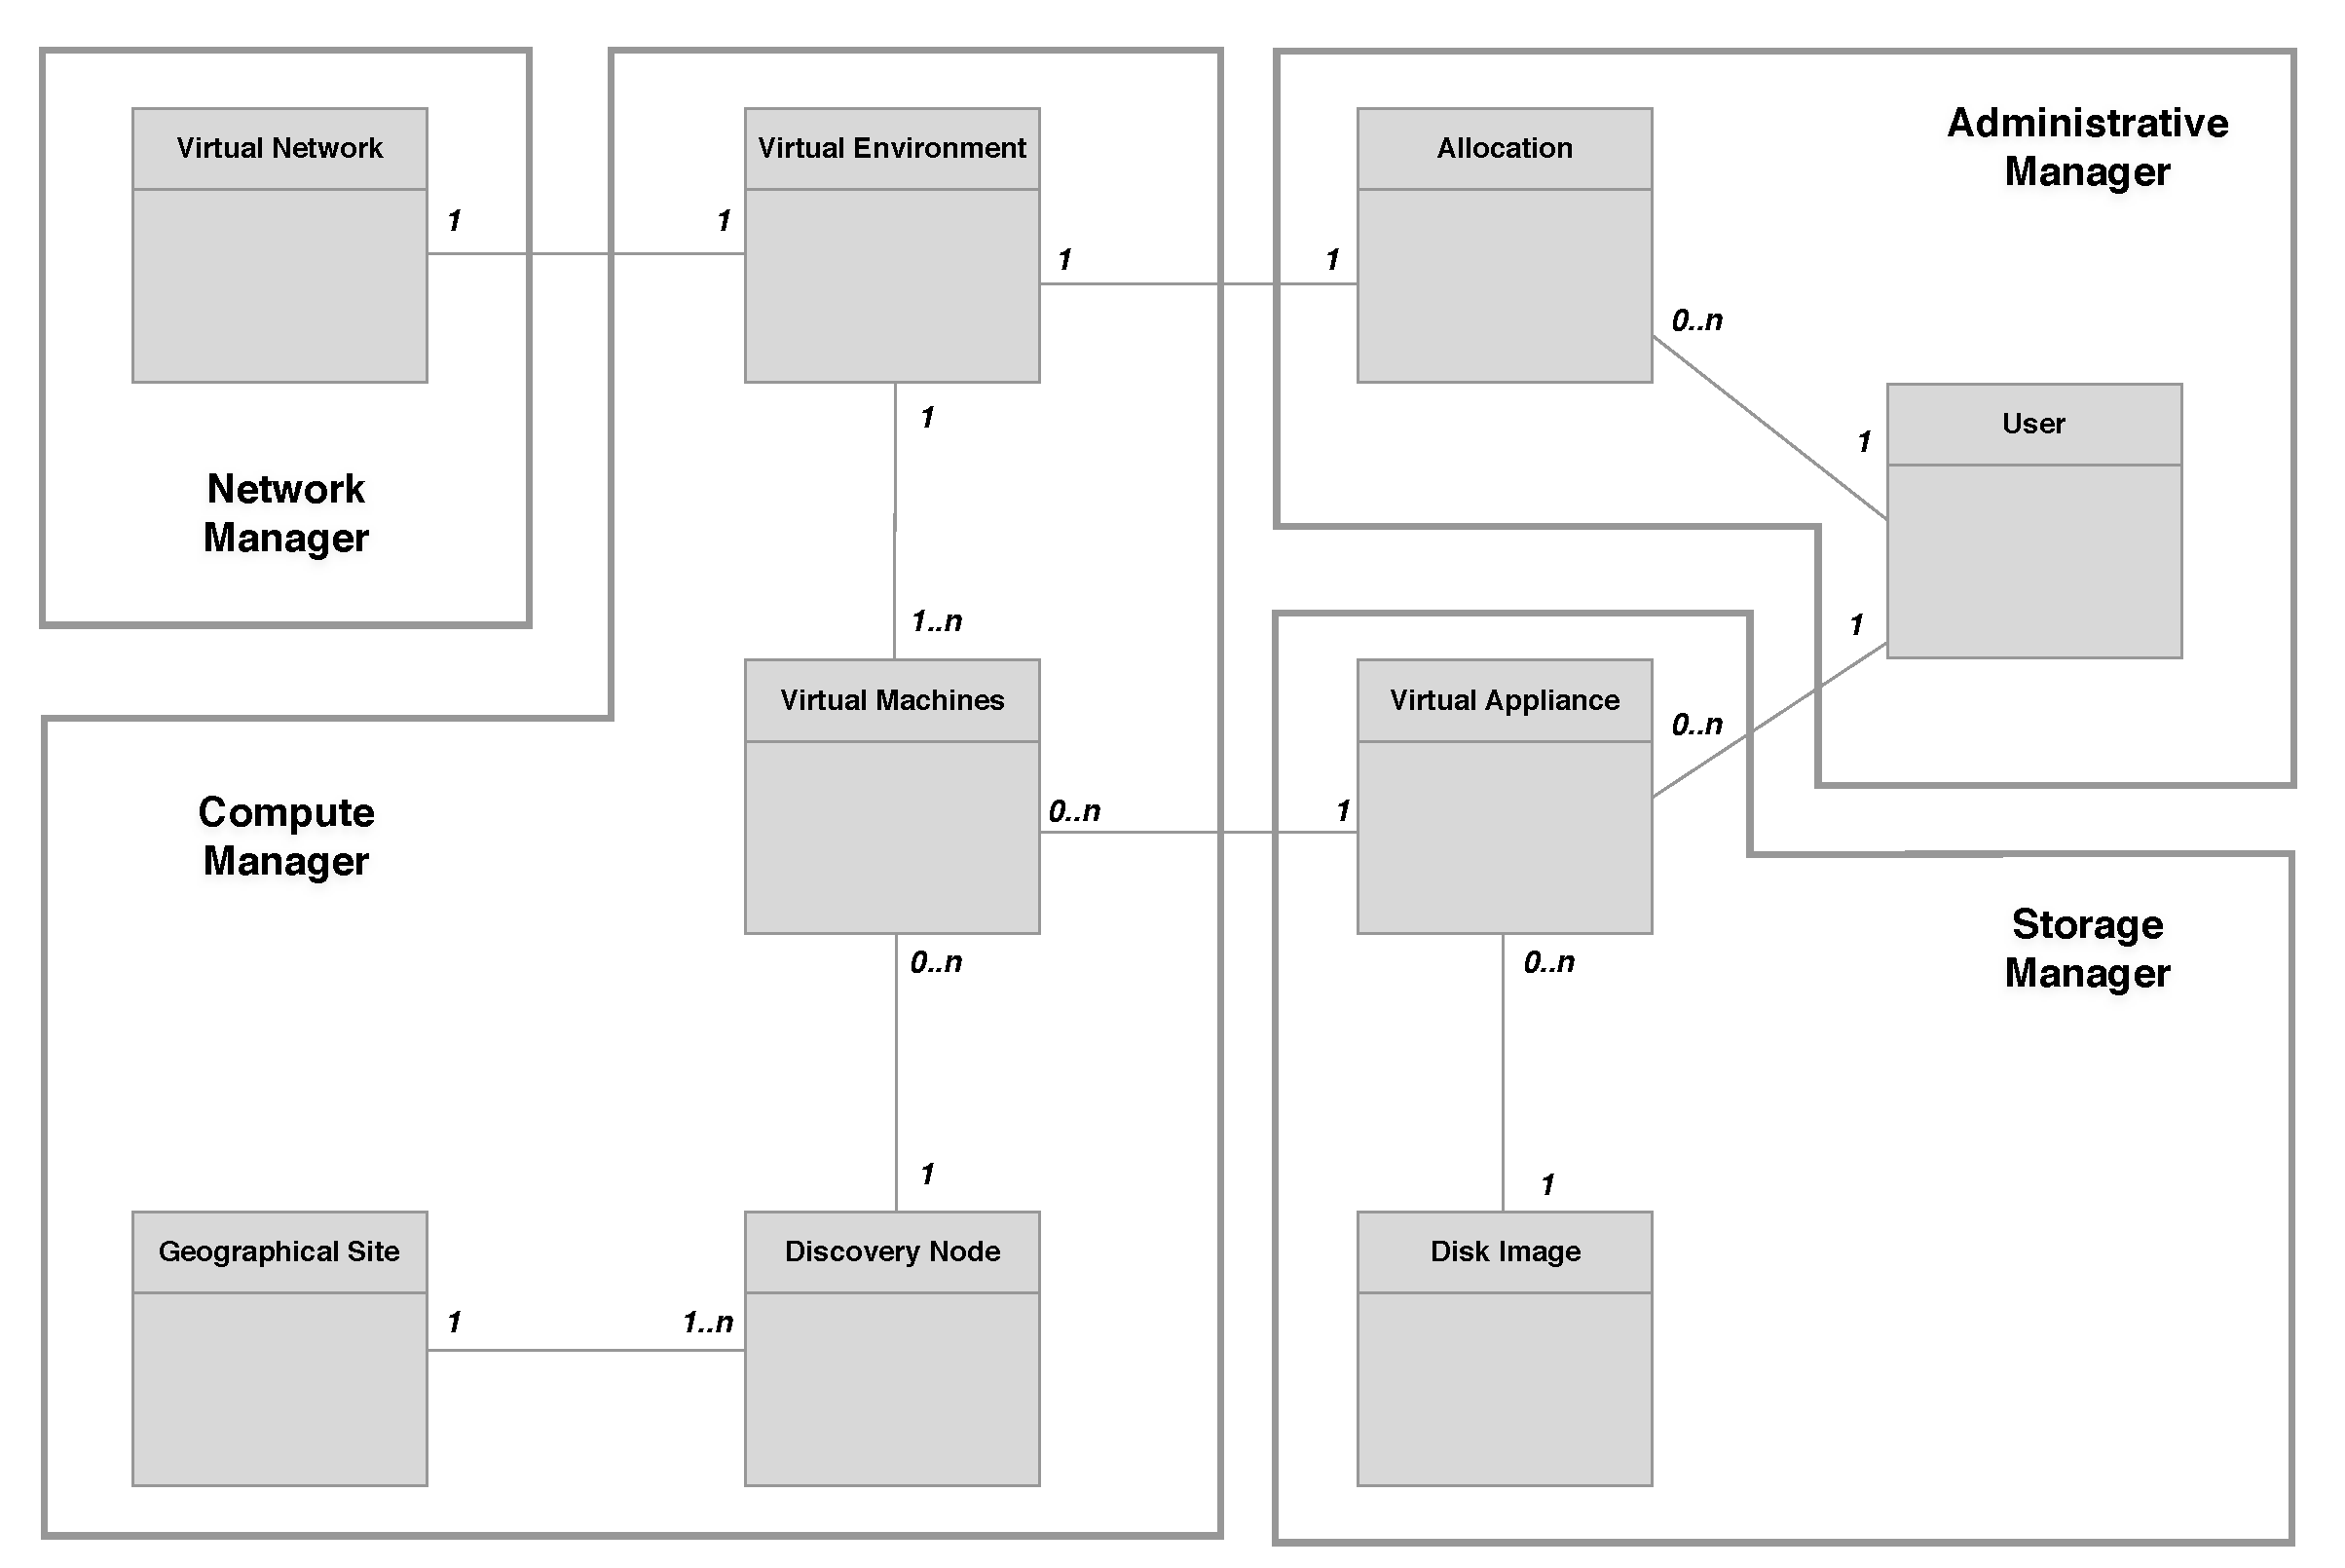
\includegraphics[width=0.91\linewidth]{Figures/mcd_3.pdf}
	\caption{Conceptual schema of the Discovery proposal.}%
	\label{fig:mcd}%
	%\vspace*{-.8cm}
\end{figure*}

In section \ref{cloud_os_concepts} fundamental concepts for the LUC-OS have been
adressed. Leveraging these concepts, we propose a first draft of the LUC-OS
architecture that focus on fundamental services. Each of these services deals 
with one concept from section \ref{cloud_os_concepts} and is described in the 
following listing:

\label{sub:sec:list_services}

\begin{description}

	\item [Compute service] : manages virtual machines' lifecycle.

	\item [Network service] : manages virtual networks.

	\item [Storage service] : manages images and block storage.

	\item [Administrative service] : manages infrastructure and users' permissions.  

\end{description}

In figure \ref{fig:mcd} we propose a conceptual schema that enables an easier 
illustration of data entities with their relationships, that we plan to use in
the LUC-OS. This is a high-level description which aims at defining and 
explaining semantics of our proposal. It is noticeable that this schema is 
partitioned in four block corresponding to the four services previously exposed.

As entities that will be manipulated by services of the LUC-OS are known, an
overview of how entities are involved during virtual machines provisioning can
be given:

\begin{itemize}

	\item A user asks the LUC-OS to provision some computing resources at a 
	specified date:  the \textbf{administrative service} considers the demand 
	and determine  wether it is possible to provide requested resources or not. 
	Once the demand is considered as acceptable, an allocation is created and 
	stored in the  LUC-OS's data structure (a Distributed Hash Table). To enable
	accounting operations such as billing, the allocation will be stored long
	enough.

	\item Once the allocation date has been reached, the \textbf{compute
	service} will ask the ressource scheduler (DVMS) to elect a 
	set of servers that is suitable to spawn the virtual machines, leading to 
	the creation of a new virtual environment which is distributed on the 
	elected servers. \textbf{Network service} then create a new virtual	network
	that is attached to the virtual	environment: during their creations, virtual
	machines will be inter-connected through this virtual network.

	\item The \textbf{storage service} is involved in processes for creating and 
	snapshotting virtual machines. As virtual machine are created from a virtual
	disk image, users will have to specify a virtual appliance (a disk image 
	base flavoured with some pre-installed software). Once a virtual machine is 
	started, it is possible for users to snapshot it: the virtual machine state
	is saved in the distributed data structure.

\end{itemize}







